\section{Motivation}
\label{sec:motivation}

We present the use case of a simplified to-do list application. Also, we take this use case as an opportunity to showcase the functionality and features of \dsl{}.

\subsection{Running Example}

The application has two screens: a main screen and a menu screen. The main screen contains a navigation bar and three to-do items. An overview of the application is given in Figure~\ref{fig:appOverview}.

\begin{figure}[!htbp]
\centering
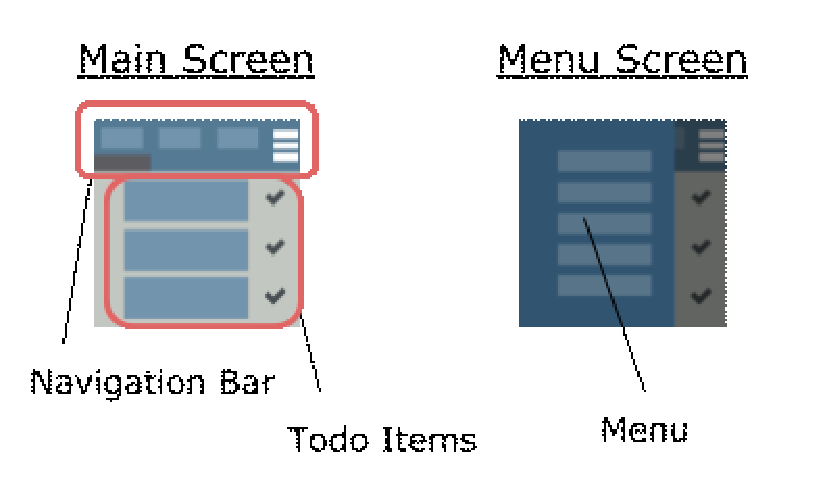
\includegraphics[width=\figscale\textwidth]{pictures/app_overview}
\caption{Overview of the to-do list application.}
\label{fig:appOverview}
\end{figure}

In this application, various user actions are accompanied with an animation:
\begin{itemize}
\item Each to-do item can be marked as \emph{done} or \emph{not done} by clicking on it. The checkmark icon changes shape and color to indicate the change in status. These are the \hs{markAsDone}/\hs{markAsNotDone} animations, of which \hs{markAsDone} is shown in Figure~\ref{fig:completeIconCheck}.
\item To-do items can be filtered by their status by using the navigation bar buttons. The first button shows all items, the second shows all complete items, and the third shows all incomplete items. Both the navigation bar underline and the to-do items itself change shape to indicate the change in selection. These are the \hs{showAll}/\hs{onlyDone}/\hs{onlyNotDone} animations, of which \hs{onlyDone} is shown in Figure~\ref{fig:onlyDoneFig}.
\item The menu screen shows/hides itself after clicking the hamburger icon. The menu expands inward from the left, to indicate the change in application state. These are the \hs{menuIntro}/\hs{menuOutro} animations, of which \hs{menuIntro} is shown in Figure~\ref{fig:menuIntroFig}.
\end{itemize}

\begin{figure}[!htbp]
\centering

\begin{subfigure}[h]{\textwidth}
\centering
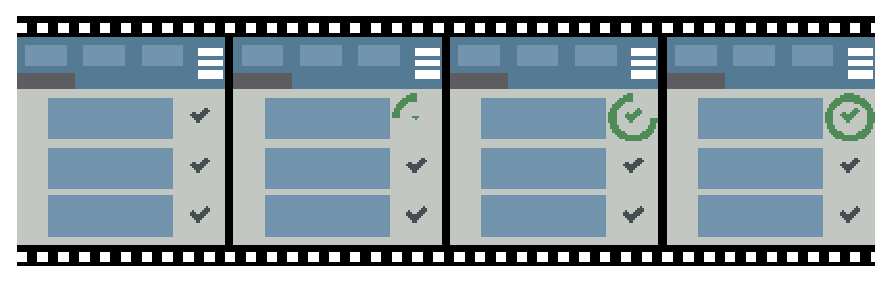
\includegraphics[width=\figscale\textwidth]{pictures/completeIconCheckFig}
\caption{The \hs{markAsDone} animation, the checkmark changes shape and color.}
\label{fig:completeIconCheck}
\end{subfigure}

\begin{subfigure}[h]{\textwidth}
\centering
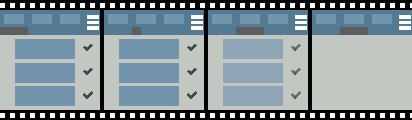
\includegraphics[width=\figscale\textwidth]{pictures/onlyDoneFig}
\caption{The \hs{onlyDone} animation, each of the not done to-do items fades out and the navbar underline changes.}
\label{fig:onlyDoneFig}
\end{subfigure}

\begin{subfigure}[h]{\textwidth}
\centering
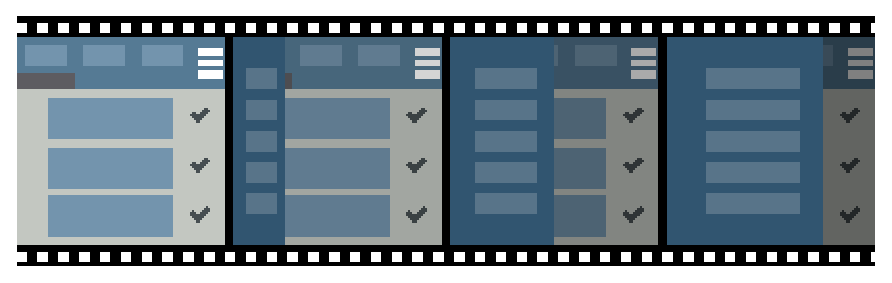
\includegraphics[width=\figscale\textwidth]{pictures/menuIntroFig}
\caption{The \hs{menuIntro} animation, the menu appears while the background fades out.}
\label{fig:menuIntroFig}
\end{subfigure}

\caption{Micro-Animations in the to-do list application.}
\label{fig:animExamples}
\end{figure}

\subsection{Composing Animations}

In \dsl{} we express animations by composing smaller animations into larger ones. When creating an animation, we need to think of a suitable decomposition. For example, the \hs{menuIntro} animation both introduces the menu screen and fades out the background. Thus, it is composed of two basic animations \hs{menuSlideIn} and \hs{appFadeOut} in parallel. The next sections explain how to construct such basic and composed animations.

\subsection{Basic Animations}

A basic animation changes the property of an element over a period of time. To specify a basic animation we need three elements: a lens specifying which property to change, the duration of the animation, and lastly the target value for this property. Since this operation creates an animation which moves a property \emph{to} a target linearly, it is called \hs{linearTo}. The duration is specified with the \hs{For} constructor while the target value is specified with the \hs{To} constructor.

\paragraph{Note on Lenses} We utilize the lens notation \texttt{x . y . z} to target the property \texttt{z} inside a nested structure \hs{{ x: { y: { z: Property } } }}. This type of lenses was introduced by Twan van Laarhoven \cite{vlLenses}, and newer versions of this idea have been packaged into various Haskell libraries, such as \texttt{lens}\footnote{\url{https://hackage.haskell.org/package/lens}}.

To implement the navigation bar underline animation, we reduce the underline width of the first button for 0.25 seconds and increase the underline width of the second button for 0.25 seconds. These animations are expressed in respectively \hs{line1Out} and \hs{line2In} below, and shown visually in Figure~\ref{fig:basic}.

\begin{spec}
line1Out = linearTo (navbar . underline1 . width) (For 0.25) (To 0)
line2In = linearTo (navbar . underline2 . width) (For 0.25) (To 28)
\end{spec}

Other examples are the \hs{menuSlideIn} and \hs{appFadeOut} animations. For the former, we increase the width of the menu over a duration of 0.5 seconds, and for the latter we increase the alpha value of the obscuring box over a duration of 0.5 seconds. These animations are shown visually in Figure~\ref{fig:basic}.

\begin{spec}
menuSlideIn = linearTo (menu . width) (For 0.5) (To 75)
appFadeOut = linearTo (obscuringBox . alpha) (For 0.5) (To 0.65)
\end{spec}

\begin{figure}[!htbp]
\centering

\begin{subfigure}[h]{\textwidth}
\centering
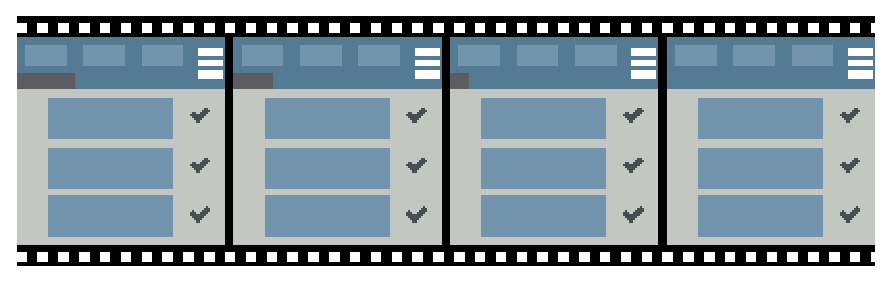
\includegraphics[width=\figscale\textwidth]{pictures/line1OutroFig}
\caption{The \hs{line1Out} animation.}
\label{fig:basic1_1}
\end{subfigure}

\begin{subfigure}[h]{\textwidth}
\centering
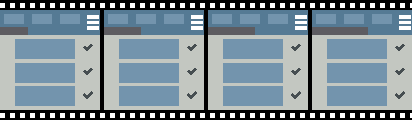
\includegraphics[width=\figscale\textwidth]{pictures/line2IntroFig}
\caption{The \hs{line2In} animation.}
\label{fig:basic1_2}
\end{subfigure}

\begin{subfigure}[h]{\textwidth}
\centering
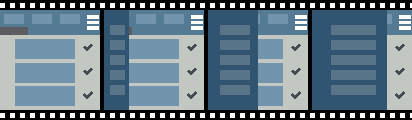
\includegraphics[width=\figscale\textwidth]{pictures/menuSlideInFig}
\caption{The \hs{menuSlideIn} animation.}
\label{fig:basic2_1}
\end{subfigure}

\begin{subfigure}[h]{\textwidth}
\centering
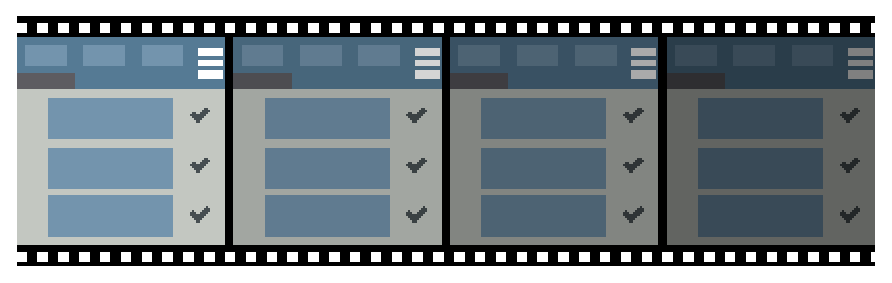
\includegraphics[width=\figscale\textwidth]{pictures/appFadeOutFig}
\caption{The \hs{appFadeOut} animation.}
\label{fig:basic2_2}
\end{subfigure}

\caption{All of the defined basic animations.}
\label{fig:basic}
\end{figure}

\subsection{Composed Animations}

A composed animation combines several other animations into one new animation. We can do this either in \emph{sequence} or in \emph{parallel}.

To obtain the \hs{selectBtn2} animation, we combine both the \hs{line1Out} and \hs{line2In} animations with the \hs{sequential} combinator. This constructs a new animation which first plays the \hs{line1Out} animation, and once it is finished plays the \hs{line2In} animation.

\begin{spec}
selectBtn2Anim = line1Out `sequential` line2In
\end{spec}

To obtain the \hs{menuIntro} animation, we combine both the \hs{menuSlideIn} and \hs{appFadeOut} animations with the \hs{parallel} combinator. This constructs a new animation which plays both the \hs{menuSlideIn} and \hs{appFadeOut} animations at the same time.

\begin{spec}
menuIntro = menuSlideIn `parallel` appFadeOut
\end{spec}

Both of these animations are shown visually in Figure~\ref{fig:composed}.

\begin{figure}[!htbp]
\centering

\begin{subfigure}[h]{\textwidth}
\centering
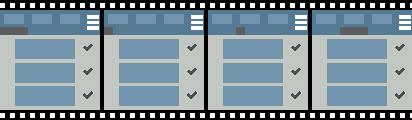
\includegraphics[width=\figscale\textwidth]{pictures/selectBtn2AnimFig}
\caption{The \hs{selectBtn2} animation.}
\label{fig:composed1}
\end{subfigure}

\begin{subfigure}[h]{\textwidth}
\centering
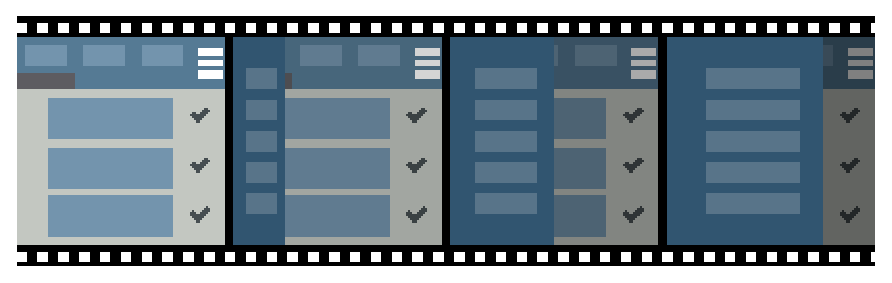
\includegraphics[width=\figscale\textwidth]{pictures/menuIntroFig}
\caption{The \hs{menuIntro} animation.}
\label{fig:composed2}
\end{subfigure}

\caption{All of the defined composed animations.}
\label{fig:composed}
\end{figure}
